
The punch benchmark is one of the few boundary value problems involving plastic solids for which there exists an exact solution. 
Such solutions are usually either for highly simplified geometries (spherical or axial symmetry, for instance) or simplified material models (such as rigid plastic solids) \cite{kacha04}.

In this experiment, a rigid punch indents a rigid plastic half space; the slip line field theory gives 
exact solutions as shown in Fig. \ref{fig_punch}a. 
The plane strain formulation of the equations and the detailed solution to the problem were derived in the Appendix of \cite{thfb08} and are also presented in \cite{gepd98}.

The two dimensional punch problem has been extensively studied numerically for the past 40 years 
\cite{zihl75,zihp95,chpe01,chan99,huhy99,yuti06,bufs08,raab07} and has been used to draw a parallel with the tectonics of eastern China in the context of the 
India-Eurasia collision \cite{tamo76,mota77}.
It is also worth noting that it has been carried out in one form or another in series of 
analogue modelling articles 
concerning the same region, with a rigid indenter colliding with a rheologically stratified lithosphere \cite{peta88,daco88,jodc90}.

 
Numerically, the one-time step punch experiment is performed on a two-dimensional
domain of purely plastic von Mises material. 
Given that the von Mises rheology yield criterion does not depend on pressure, the density of the material and/or the gravity vector is set to zero. Sides are set to free slip boundary conditions, the bottom to no slip, while a vertical velocity $(0,-v_p)$ is prescribed at the top boundary for nodes whose $x$ coordinate is within $[L_x/2-\delta/2,L_x/2+\delta/2]$. 

The following parameters are used: $L_x=1$, $L_y=0.5$, $\mu_{min}=10^{-3}$, 
$\mu_{max}=10^3$, $v_p=1$, $\delta=0.123456789$ 
and the yield value of the material is set to $k=1$. 

The analytical solution predicts that the angle of the shear bands stemming from the sides of the punch 
is $\pi/4$, that the pressure right under the punch is $1+\pi$, 
and that the velocity of the rigid blocks on each side of the punch is $v_p/\sqrt{2}$ 
(this is simply explained by invoking conservation of mass).

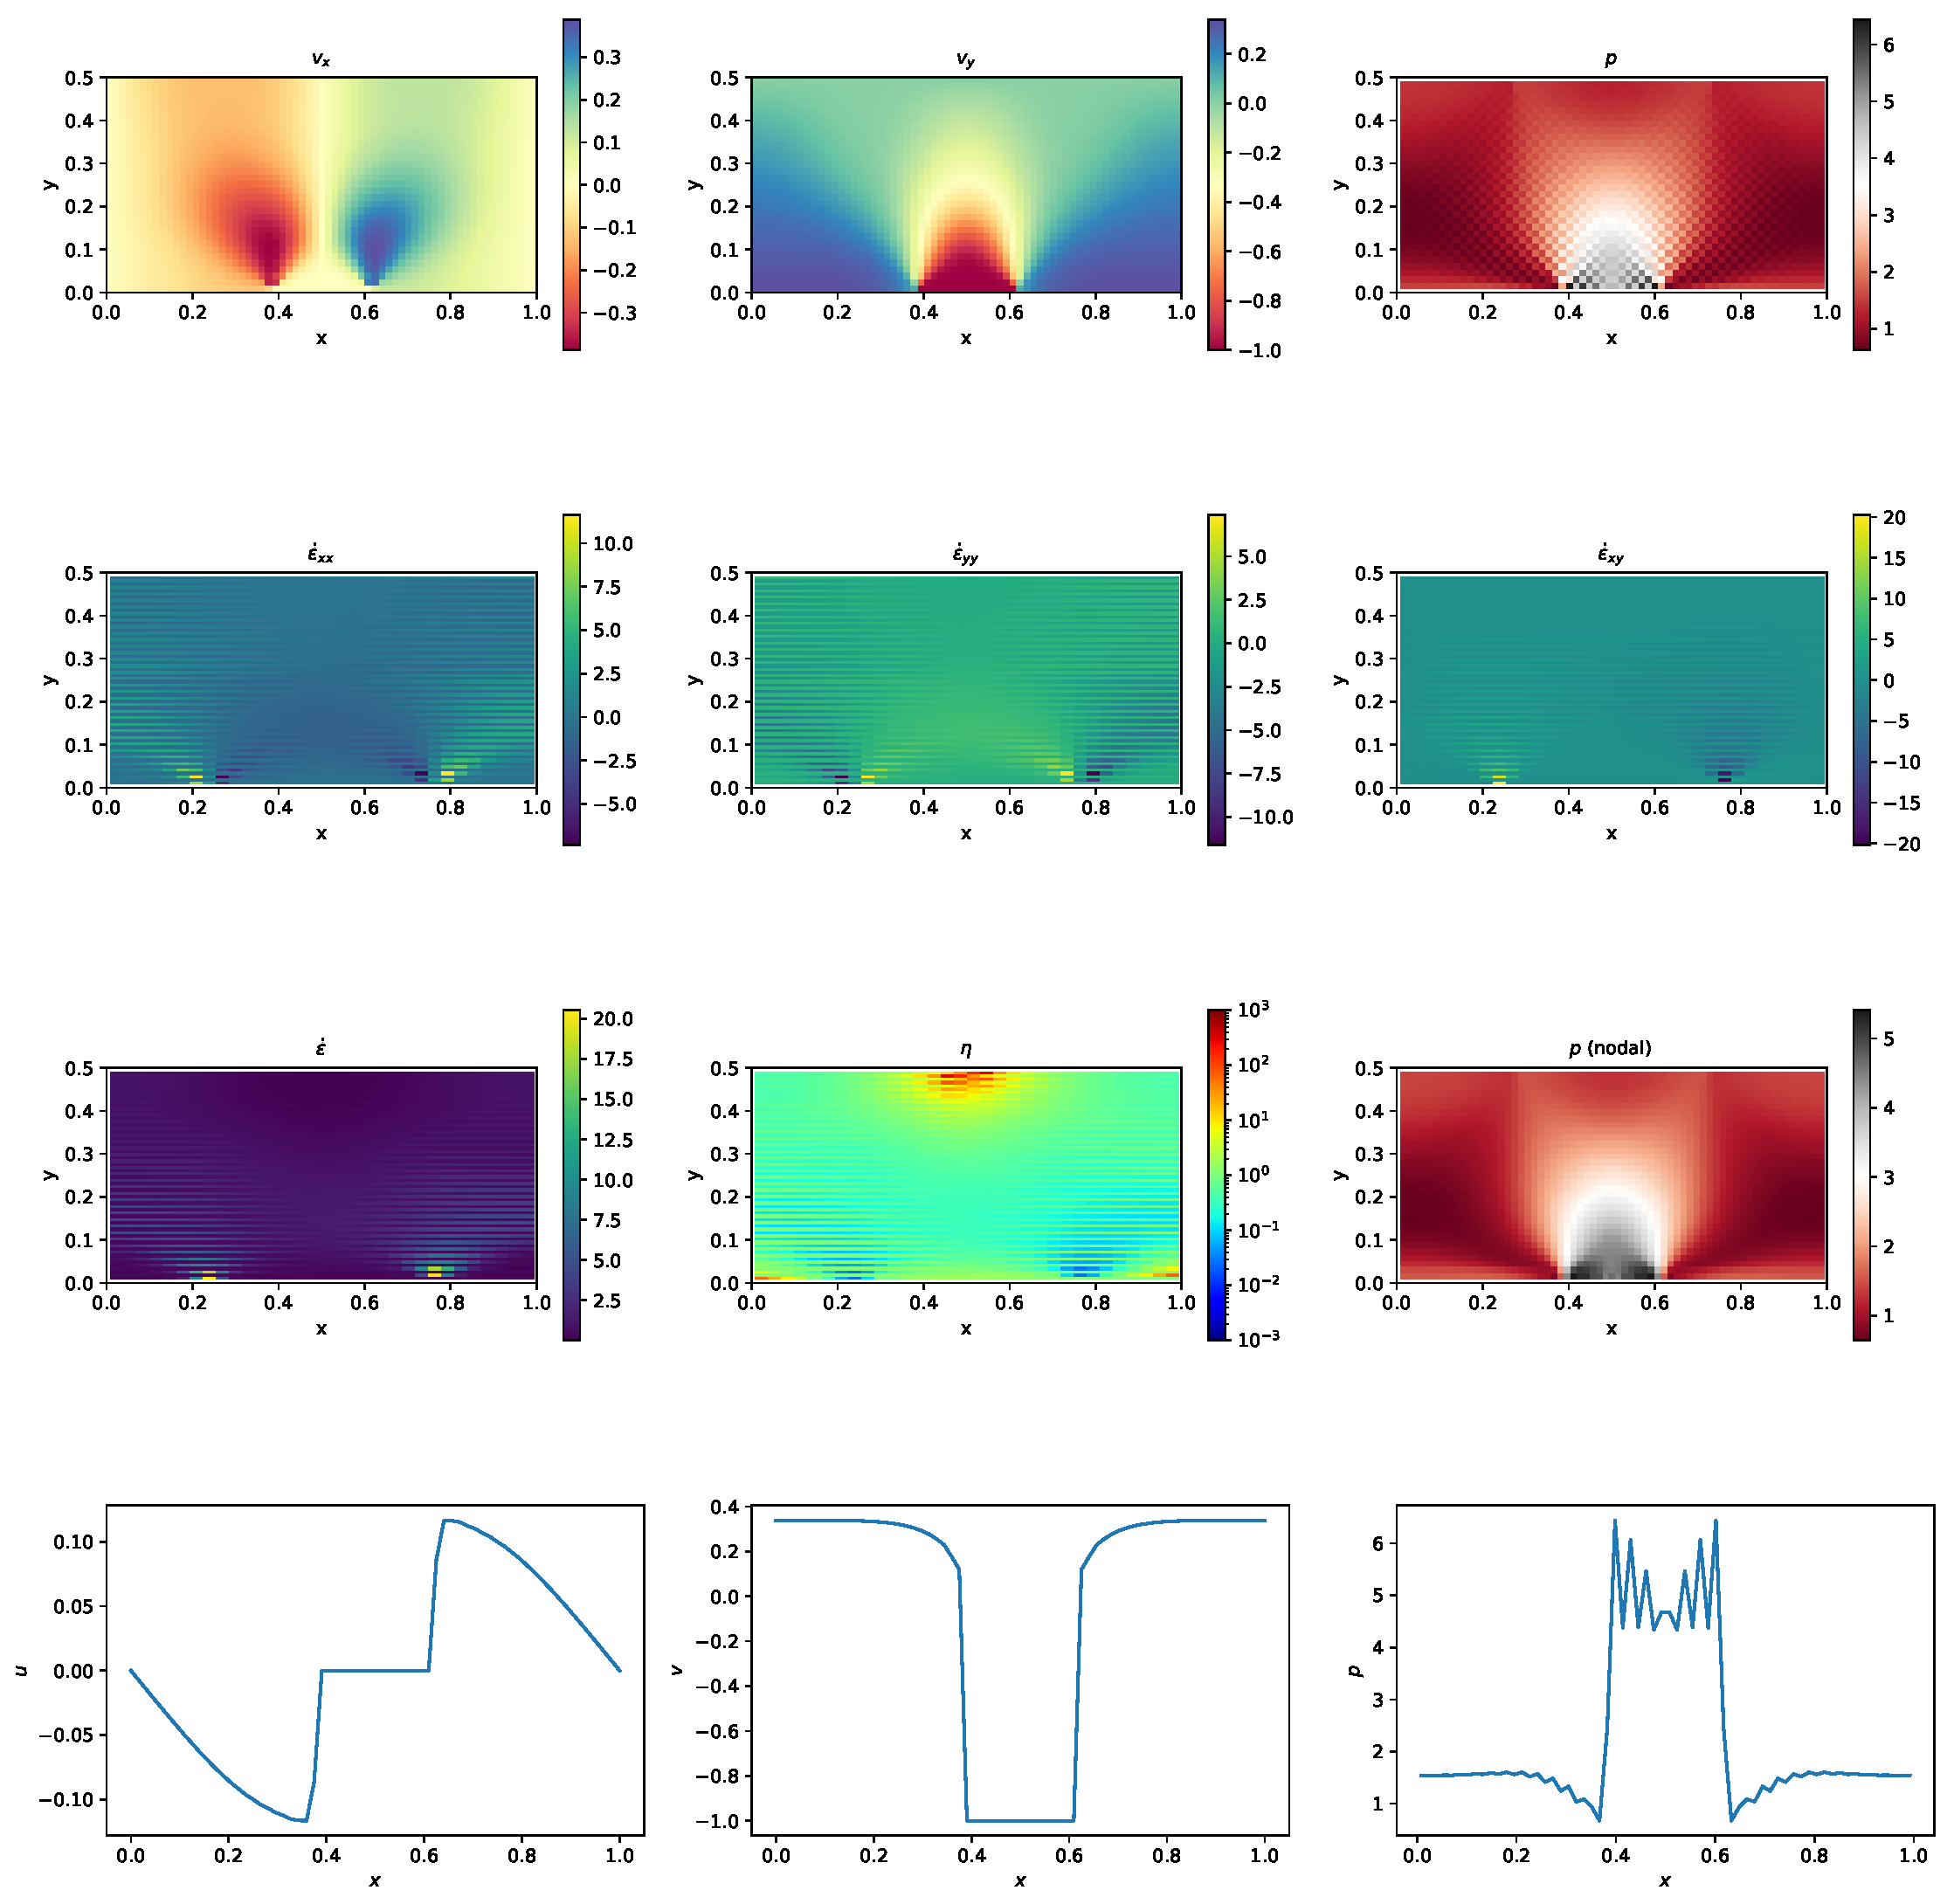
\includegraphics[width=16cm]{python_codes/fieldstone_08/solution.pdf}

ToDo: smooth punch

\fbox{
\parbox{10cm}{{\bf features}
\begin{itemize}
\item $Q_1\times P_0$ element \index{$Q_1 \times P_0$}
\item incompressible flow \index{incompressible flow}
\item penalty formulation \index{penalty formulation}
\item Dirichlet boundary conditions (no-slip)
\item isothermal \index{isothermal}
\item non-isoviscous \index{non-isoviscous}
\item nonlinear rheology \index{nonlinear rheology}
\end{itemize}
}}

